%----------------------------------------------------------------------------------------
%	PACKAGES AND OTHER DOCUMENT CONFIGURATIONS
%----------------------------------------------------------------------------------------

\documentclass[paper=a4, fontsize=11pt]{scrartcl} % A4 paper and 11pt font size

\usepackage[T1]{fontenc} % Use 8-bit encoding that has 256 glyphs
\usepackage{fourier} % Use the Adobe Utopia font for the document - comment this line to return to the LaTeX default
%\usepackage{palatino}
\usepackage[english]{babel} % English language/hyphenation
\usepackage{amsmath,amsfonts,amsthm} % Math packages

\usepackage{enumerate}
\usepackage{listings}  % Use this for better code formatting
%\usepackage{xcolor} 
\usepackage{graphicx}    
\usepackage[svgnames]{xcolor} 

%\usepackage{sectsty} % Allows customizing section commands
%\allsectionsfont{\centering \normalfont\scshape} % Make all sections centered, the default font and small caps
 \usepackage{setspace} 
 
\usepackage{fancyhdr} % Custom headers and footers
\pagestyle{fancyplain} % Makes all pages in the document conform to the custom headers and footers
\fancyhead{} % No page header - if you want one, create it in the same way as the footers below
\fancyfoot[L]{} % Empty left footer
\fancyfoot[C]{} % Empty center footer
\fancyfoot[R]{\thepage} % Page numbering for right footer
\renewcommand{\headrulewidth}{0pt} % Remove header underlines
\renewcommand{\footrulewidth}{0pt} % Remove footer underlines
\setlength{\headheight}{13.6pt} % Customize the height of the header
\setlength{\parindent}{0cm}
\setlength{\parskip}{.1cm plus4mm minus3mm}


%--- color definitions for code listings
\definecolor{mygreen}{rgb}{0,0.6,0}
\definecolor{mygray}{rgb}{0.5,0.5,0.5}
\definecolor{mymauve}{rgb}{0.58,0,0.82}


% commands I use to typeset matrices in bold
\newcommand{\matLambda}{\mathbf{\Lambda}}
\newcommand{\matSigma}{\mathbf{\Sigma}}
\newcommand{\vecBeta}{\mathbf{\beta}}
\newcommand{\vecEpsilon}{\mathbf{\epsilon}}
\newcommand{\vecMu}{\mathbf{\mu}}
\newcommand{\vecY}{\mathbf{y}}
\newcommand{\matA}{\mathbf{A}}
\newcommand{\matB}{\mathbf{B}}
\newcommand{\matC}{\mathbf{C}}
\newcommand{\matI}{\mathbf{I}}
\newcommand{\matP}{\mathbf{P}}
\newcommand{\matS}{\mathbf{S}}
\newcommand{\matV}{\mathbf{V}}
\newcommand{\matQ}{\mathbf{Q}}
\newcommand{\matX}{\mathbf{X}}
\newcommand{\matY}{\mathbf{Y}}
\newcommand{\matW}{\mathbf{W}}



%\numberwithin{equation}{section} % Number equations within sections (i.e. 1.1, 1.2, 2.1, 2.2 instead of 1, 2, 3, 4)
%\numberwithin{figure}{section} % Number figures within sections (i.e. 1.1, 1.2, 2.1, 2.2 instead of 1, 2, 3, 4)
%\numberwithin{table}{section} % Number tables within sections (i.e. 1.1, 1.2, 2.1, 2.2 instead of 1, 2, 3, 4)

%\setlength\parindent{0pt} % Removes all indentation from paragraphs - comment this line for an assignment with lots of text

%----------------------------------------------------------------------------------------
%	TITLE SECTION
%----------------------------------------------------------------------------------------

\newcommand{\horrule}[1]{\rule{\linewidth}{#1}} % Create horizontal rule command with 1 argument of height

\title{	
\normalfont \normalsize 
%\textsc{stat 8004} \\ [25pt] 
\horrule{0.5pt} \\[0.4cm] % Thin top horizontal rule
\huge STAT 8004, Assignment 3 \\ % The assignment title
\horrule{2pt} \\[0.5cm] % Thick bottom horizontal rule
}

\author{David Dobor} 

\date{\normalsize\today} % Today's date or a custom date

\lstset{ %
  language=R,                     % the language of the code
  basicstyle=\small\ttfamily,
  backgroundcolor=\color{WhiteSmoke},  % choose the background color. You must add \usepackage{color}
  showspaces=false,               % show spaces adding particular underscores
  showstringspaces=false,         % underline spaces within strings
  showtabs=false,                 % show tabs within strings adding particular underscores
  frame=single,                   % adds a frame around the code
  rulecolor=\color{Gray},        % if not set, the frame-color may be changed on line-breaks within not-black text (e.g. commens (green here))
  tabsize=2,                      % sets default tabsize to 2 spaces
  captionpos=b,                   % sets the caption-position to bottom
  breaklines=true,                % sets automatic line breaking
  breakatwhitespace=false,        % sets if automatic breaks should only happen at whitespace
  title=\lstname,                 % show the filename of files included with \lstinputlisting;
                                  % also try caption instead of title
  keywordstyle=\color{DarkSlateBlue},      % keyword style
  commentstyle=\color{ForestGreen},   % comment style
  stringstyle=\color{mymauve},      % string literal style
  %escapeinside={\%*}{*)},         % if you want to add a comment within your code
  morekeywords={*,det,...}            % if you want to add more keywords to the set
} 

\renewcommand{\ttdefault}{pcr}  %to be able to use bold fonts in lstlistings code

\begin{document}

\maketitle 

%----------------------------------------------------------------------------------------
%	PROBLEM 1
%----------------------------------------------------------------------------------------

%\section*{Problem title}

\subsection*{Question 1}
Suppose that we are working under Gauss-Markov model
$$
\matY = \matX \vecBeta + \vecEpsilon
$$
where $E (\vecEpsilon) = \mathbf{0}$ and var$(\vecEpsilon) = \sigma^2 \matI.$ Let $\hat \matY$ be the 
ordinary least square estimator of $\matY$.\\

\begin{enumerate}[(a)]
\item Show that $\hat \matY$ and $\matY - \hat \matY$ are uncorrelated.
\vspace{5mm}
\item Show that 
$$
E \{(\matY - \hat \matY)^T (\matY - \hat \matY) \} = \sigma^2 \{n - \text{rank}(\matX)\}.
$$
\end{enumerate}


\bigskip
\subsubsection*{Answer to Question 1}

\begin{enumerate}[(a)]
\item First, establish orthogohality of $\matP_X \matY = \hat \matY$ and $( \matI - \matP_X) \matY = \matY - \hat \matY$. This follows because
\begin{align*}
(\matY - \hat \matY)^T \hat \matY &=  ( ( \matI - \matP_X)  \matY )^T \hat \matY = \hat \matY^T (  ( \matI - \matP_X) ^T \matP_X ) \matY,
\end{align*}
and the middle term in the last expression is identically zero ( i.e., $ ( \matI - \matP_X) ^T \matP_X = \matP_X - \matP_X ^T \matP_X = \matP_X - \matP_X = 0$ by idempotence and symmetry of $\matP_X$).\\

Therefore
\begin{align*}
(\matY - \hat \matY)^T \hat \matY &=  0.
\end{align*}
Since in the Gauss-Markov model we also have that $E( \matY)  = \hat \matY$, it then follows that
\begin{align*}
E ( \hat \matY (\matY - \hat \matY) ) - E (\hat \matY) E( \matY - \hat \matY) =  E (0) - E (\hat \matY) \times 0 = 0.
\end{align*}
\vspace{5mm}
\item By Theorem 5.2 (a) we have that (taking the `any symmetric` $\matA$ to be $\matI$ in that theorem):
\begin{align*}
E (\vecY^T \vecY) = tr(\matSigma) + \vecMu^T \vecMu.
\end{align*}
We apply this theorem with $\matY - \hat \matY$ for $\vecY$, whose `$\vecMu$` in the Gauss-Markov model is $0$.
Thus since
\begin{align*}
\text{var}(\matY - \hat \matY) = \text{var}(\ (\matI - \matP_X)  \matY \ ) = \sigma^2 (\matI - \matP_X) ,
\end{align*}
and 
$$
tr(\matSigma) = tr(\sigma^2 (\matI - \matP_X) ) = \sigma^2 (tr(\matI) - tr(\matP_X)) = \sigma^2 (n - \text{rank(X)}),
$$
the result follows.
\end{enumerate}

\bigskip
\bigskip
%----------------------------------------------------------------------------------------
%	PROBLEM 2
%----------------------------------------------------------------------------------------

\subsection*{Question 2}
Consider the one-way \texttt{ANOVA} model $y_{ij} = \mu + \tau_i + \epsilon_{ij}$ for the $j$th 
individual of the $i$th group. Suppose there are 4 treatments (groups) and the sample sizes are 
respectively 2,1,1,2 for treatments. Now suppose that $\matY = (y_{11}, y_{12}, y_{21}, y_{31}, y_{41}, y_{42})^T = (2, 1, 4, 6, 3, 5)^T$ contains the observations. 
Use \texttt{R} and weighted generalized least squares to find appropriate estimate for\\

$$
E (\matY)  \text{ \  and \  } 
\begin{bmatrix} 1 & 1 & 0 & 0 & 0 \\
                             1 & 0 & 1 & 0 & 0 \\
                             1 & 0 & 0 & 1 & 0 \\
                             1 & 0 & 0 & 0 & 1 \\
\end{bmatrix}
\vecBeta
$$

in the Aiken model with $\text{var}(\vecEpsilon) = \matV$ for two cases where

\begin{enumerate}[(a)]
\item $\matV = \matV_1 = \text{diag}(1, 9, 9, 1, 1, 9)$ and
\item 
$$
\matV = \matV_2 = 
\begin{bmatrix} 1 & 1 & 0 & 0 & 0 & 0 \\
                             1 & 9 & 0 & 0 & 0 & 0 \\
                             0 & 0 & 9 & -1 & 0 & 0 \\
                             0 & 0 & -1 & 1 & 0 & 0 \\
                             0 & 0 & 0 & 0 & 1 & -1 \\
                             0 & 0 & 0 & 0 & -1 & 9 \\
\end{bmatrix}
$$
\end{enumerate}

\bigskip
\subsubsection*{Answer to Question 2}

\bigskip
\bigskip
%----------------------------------------------------------------------------------------
%	ANSWER TO PROBLEM 2
%----------------------------------------------------------------------------------------
In what follows we transform the following Aiken model
$$
\begin{bmatrix} 
2\\ 1\\ 4 \\ 6 \\ 3\\ 5  
\end{bmatrix}
=
\begin{bmatrix} 1 & 1 & 0 & 0 & 0 \\
                             1 & 1 & 0 & 0 & 0 \\
                             1 & 0 & 1 & 0 & 0\\
                             1 & 0 & 0 & 1 & 0 \\
                             1 & 0 & 0 & 0 & 1\\
                             1 & 0 & 0 & 0 & 1
\end{bmatrix}
\begin{bmatrix} 
\mu \\ \tau_1\\ \tau_2 \\ \tau_3 \\ \tau_4 \\ 
\end{bmatrix}
+ 
\begin{bmatrix} 
\epsilon_{1 1 } \\ \epsilon_{1 2}\\ \epsilon_{2 1} \\ \epsilon_{3 1} \\ \epsilon_{4 1} \\\epsilon_{42}  
\end{bmatrix}
$$

to the Gauss-Markov model with an appropriate linear transformation. We do the \texttt{OLS} estimation
as usual in the resulting Gauss-Markov model. We then transform our estimates back to the `Aiken-space` and report the results. 
\pagebreak
\begin{enumerate}[(a)]
\item 
\begin{lstlisting}[basicstyle=\ttfamily\small\bfseries]
library(MASS) # function ginv() is in the MASS library
# data given in problem 2:
X <- matrix( 
    c(1, 1, 1, 1, 1, 1, 
      1, 1, 0, 0, 0, 0,
      0, 0, 1, 0, 0, 0,
      0, 0, 0, 1, 0, 0, 
      0, 0, 0, 0, 1, 1 ), 
    nrow=6, 
    ncol=5) 

y <- matrix(c(2, 1, 4, 6, 3, 5), 6, 1)

# error variance 
V1 <- diag(c(1, 9, 9, 1, 1, 9));
V1.inv <- solve(V1);
# transformation to convert Aiken to Gauss-Markov:
V1.inv.sqrt = sqrt(V1.inv);

# transform data with V1.inv.sqrt:
u <- V1.inv.sqrt %*% y
W <- V1.inv.sqrt %*% X

# beta.hat in the transformed model:
beta.hat <- ginv(t(W) %*% W) %*% t(W) %*% u

# compute u.hat
u.hat <- W %*% beta.hat

# back to y.hat
y.hat <- solve(V1.inv.sqrt) %*% u.hat

## The estimate of c^T \beta
c.t <- matrix( 
    c(1, 1, 1, 1, 
      1, 0, 0, 0,
      0, 1, 0, 0,
      0, 0, 1, 0,
      0, 0, 0, 1), 
    nrow=4, 
    ncol=5) 

c.t %*% ginv(t(W) %*% W) %*% t(W) %*% u

\end{lstlisting}

\pagebreak
The output for $\hat y$:
\begin{lstlisting}[basicstyle=\ttfamily\small\bfseries]
> y.hat
     [,1]
[1,]  1.9
[2,]  1.9
[3,]  4.0
[4,]  6.0
[5,]  3.2
[6,]  3.2
\end{lstlisting}

The output for the estimate of $ c^T  \beta $:
\begin{lstlisting}[basicstyle=\ttfamily\small\bfseries]
     [,1]
[1,]  1.9
[2,]  4.0
[3,]  6.0
[4,]  3.2
\end{lstlisting}



\item 

\begin{lstlisting}[basicstyle=\ttfamily\small\bfseries]
V2 <- matrix( 
    c(1,  1,   0,   0,  0,  0,
      1,  9,   0,   0,  0,  0,
      0,  0,   9,  -1,  0,  0,
      0,  0,  -1,   1,  0,  0,
      0,  0,   0,   0,  1, -1,
      0,  0,   0,   0, -1,  9),
    nrow=6, 
    ncol=6) 

# first, compute the inverse square root of V2
Q <- eigen(V2)$vectors              
# D contains the inverse square roots of of V's eigenvalues 
# on the diagonal, zeros elsewhere:
D <- diag(1/sqrt(eigen(V2)$values))

# The desired `inverse square root` matrix.
# It's the transformation to convert Aiken to Gauss-Markov:
V2.inv.sqrt <- Q %*% D %*% t(Q)  

# transform data with V2.inv.sqrt:
u <- V2.inv.sqrt %*% y
W <- V2.inv.sqrt %*% X

# beta_hat in the transformed model:
beta.hat <- ginv(t(W) %*% W) %*% t(W) %*% u

# compute u.hat
u.hat <- W %*% beta.hat

# back to y.hat
y.hat <- solve(V2.inv.sqrt)%*% u.hat

## The estimate of c^T \beta
c.t %*% ginv(t(W) %*% W) %*% t(W) %*% u
\end{lstlisting}


Output for $\hat y$:

\begin{lstlisting}[basicstyle=\ttfamily\small\bfseries]
> y.hat
      [,1]
[1,] 2.000
[2,] 2.000
[3,] 4.000
[4,] 6.000
[5,] 3.333
[6,] 3.333
\end{lstlisting}

The output for the estimate of $ c^T  \beta $:
\begin{lstlisting}[basicstyle=\ttfamily\small\bfseries]
      [,1]
[1,] 2.000
[2,] 4.000
[3,] 6.000
[4,] 3.333
\end{lstlisting}
\end{enumerate}



\pagebreak
%----------------------------------------------------------------------------------------
%	PROBLEM 3
%----------------------------------------------------------------------------------------

\subsection*{Question 3}
The \texttt{lm} function in \texttt{R} allows one to do weighted least squares with the form
$\sum w_i (y_i - \hat y_i)^2$ for positive weights $w_i$. For $\matV_1$ in the last question,
find the \texttt{BLUE}s of the 4 cell means using \texttt{lm} and an appropriate vector of weights.

\bigskip
\subsubsection*{Answer to Question 3}

\begin{lstlisting}[basicstyle=\ttfamily\small\bfseries]
X <- matrix( 
    c(1, 1, 1, 1, 1, 1, 
      1, 1, 0, 0, 0, 0,
      0, 0, 1, 0, 0, 0,
      0, 0, 0, 1, 0, 0, 
      0, 0, 0, 0, 1, 1 ), 
    nrow=6, 
    ncol=5) 

y <- matrix(c(2, 1, 4, 6, 3, 5), 6, 1)

lm(y ~ X[,2:5] -1, weights=c(1, 1/9, 1/9, 1, 1, 1/9))
\end{lstlisting}
output agrees with question 2:
\begin{lstlisting}[basicstyle=\ttfamily\small\bfseries]
Call:
lm(formula = y ~ X[, 2:5] - 1, weights = c(1, 1/9, 1/9, 1, 1, 
    1/9))

Coefficients:
X[, 2:5]1  X[, 2:5]2  X[, 2:5]3  X[, 2:5]4  
      1.9        4.0        6.0        3.2  
\end{lstlisting}


\pagebreak
%----------------------------------------------------------------------------------------
%	PROBLEM 4
%----------------------------------------------------------------------------------------

\subsection*{Question 4}
Running
\begin{lstlisting}[basicstyle=\ttfamily\small\bfseries]
library (MASS)
data(Boston)
\end{lstlisting}
will load the \texttt{Boston} housing data into\texttt{R}. Use \texttt{?Boston} to see the information on the variables.  Now create two matrices $\matY$ and $\matX$ that will be used to fit a regression model to some of these data.\\



\begin{lstlisting}[basicstyle=\ttfamily\small\bfseries]
Y=as.matrix(Boston$medv)
X=as.matrix(Boston[,c('crim','nox','rm','age','dis')])
X=cbind(rep(1,dim(Boston)[1]),X)
\end{lstlisting}


\begin{enumerate}[(a)]

\item Make a scatterplot matrix for $y, x_1, \ldots, x_5$. If you had to guess based on this plot, which single
predictor do you think is probably the best predictor of Price? Do you see any evidence of multicollinearity (correlation among the predictors) in this graphic?

\item Use \texttt{qr()} function to find the rank of $\matX$.

\item Use \texttt{R} matrix operations on the $\matX$ matrix and $\matY$ vector to find the estimated
 regression coefficient vector $\hat \beta$, the estimated mean vector $\hat \matY$, and the vector of 
 residuals $ \mathbf{e} = \matY - \hat \matY$. 
 
\item Plot the residuals against the fitted means.

\item Create a normal plot from the values in the residual vector.

\item Compute the sum of squared residuals and the corresponding estimate of $\sigma^2$
$$
\hat \sigma^2 = \frac{(\matY - \hat \matY)^T (\matY - \hat \matY)} { n - \text{rank}(\matX)}
$$
\item Call the \texttt{lm} function in \texttt{R} and confirm your answers, and note that \texttt{?lm} gives 
you various information such as the outputs of the function.
\begin{lstlisting}[basicstyle=\ttfamily\small\bfseries]
m1=lm(medv~crim+nox+rm+age+dis,data=Boston)
\end{lstlisting}
\end{enumerate}


\subsubsection*{Answer to Question 4}


\begin{enumerate}[(a)]
\item The average number of rooms ( \texttt{rm} ) has the highest correlation with the price ( \texttt{medv} ).  

Although there is no sign of perfect multicollinearity here (after all $X$ is of full rank), some variables appear to be highly correlated. For example,  \texttt{age} and \texttt{dis} are highly negatively correlated (perhaps the discerning eye of an expert 
statistician might do better at detecting such patterns). 

\begin{center}
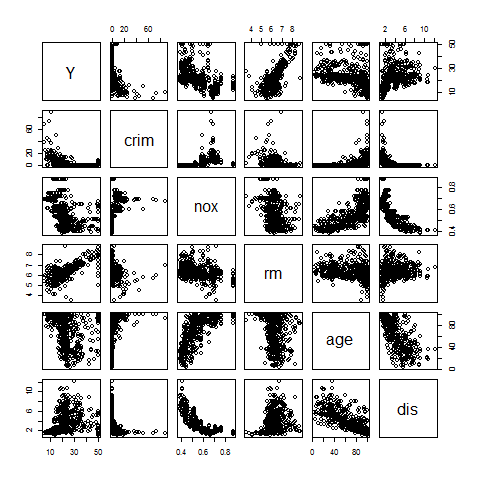
\includegraphics[width=10cm, height=12cm, width= 12cm]{scatter_a}
\end{center} 

\item
\begin{lstlisting}[basicstyle=\ttfamily\small\bfseries]
> qrx <- qr(X)
> qrx$rank
[1] 6
\end{lstlisting}
\pagebreak
\item Output for $\hat \beta$ is given below. Outputs for $\hat \matY$ and  $\mathbf{e} = \matY - \hat \matY$  are 506 elements long, so only the first few are shown.
\begin{lstlisting}[basicstyle=\ttfamily\small\bfseries]
> beta.hat <- solve(t(X) %*% X) %*% t(X) %*% Y
> beta.hat
             [,1]
      -6.22734381
crim  -0.20808251
nox  -18.05089222
rm     7.73531226
age   -0.06662411
dis   -1.19104483
\end{lstlisting}

\begin{lstlisting}[basicstyle=\ttfamily\small\bfseries]
> Y.hat <- X %*% beta.hat
> head(Y.hat)  # 506 long - show only first few
      [,1]
1 25.70437
2 23.79686
3 30.89256
4 29.35859
5 29.94388
6 24.10601
\end{lstlisting}

\begin{lstlisting}[basicstyle=\ttfamily\small\bfseries]
> e <- Y - Y.hat
> head(e)  # 506 long - show only first few
       [,1]
1 -1.704374
2 -2.196864
3  3.807444
4  4.041409
5  6.256122
6  4.593993
\end{lstlisting}
\pagebreak
\item We note the following pattern in the residuals: the points that seem to lie on a straight line from the upper left to the bottom right (result of censoring \texttt{medv} above a certain value):
   
 \begin{center} 
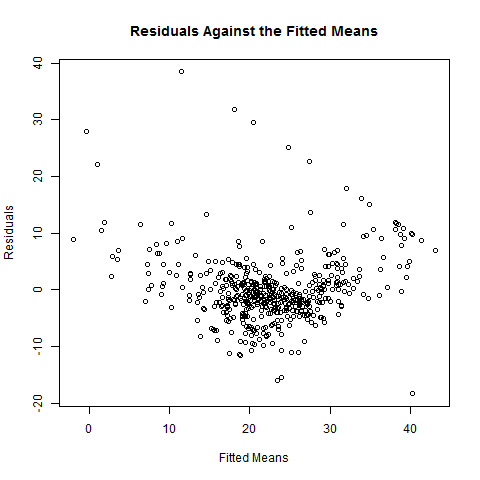
\includegraphics[width=10cm, height=10cm, width= 10cm]{resids_d}
\end{center} 

\pagebreak
\item The residuals clearly deviate from normality:
 \begin{center}
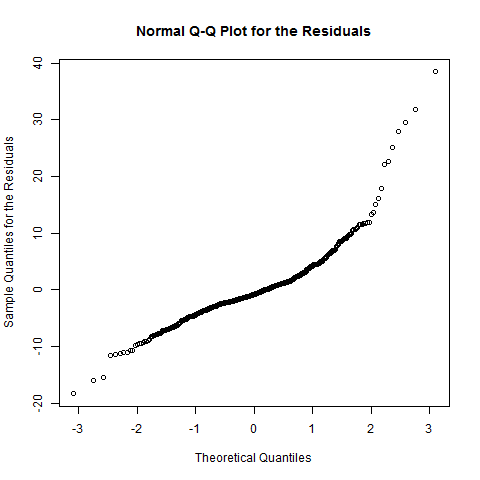
\includegraphics[width=10cm, height=10cm, width= 10cm]{normplot_e}
\end{center} 
\item   \ 

\begin{lstlisting}[basicstyle=\ttfamily\small\bfseries]
> sigma.squared.hat <- (t(e) %*% e) / (506 - 6)
> sigma.squared.hat
         [,1]
[1,] 34.82387
\end{lstlisting}

\item All the quantities computed earlier based on matrix operations can be obtained from a call to 
\texttt{lm}. For example:
\begin{lstlisting}[basicstyle=\ttfamily\small\bfseries]
m1=lm(medv~crim+nox+rm+age+dis,data=Boston)
m1$coeff           # agrees with beta.hat computed earlier
m1$residuals       # agrees with e computed earlier
m1$df.residual     # agrees with 506 - rank(X)
# etc., etc., etc..
\end{lstlisting}

\end{enumerate}












\end{document}